\documentclass{article}

\usepackage[margin=1.5in]{geometry}
\usepackage{upgreek}
\usepackage{lscape}
\usepackage{rotating}
\usepackage{amsmath}
\usepackage{tikz}
% \usepackage{graphicx}
\usepackage{graphics}
\usepackage{caption}
\usepackage{subcaption}
\usepackage{mathrsfs}
\usepackage[toc,page]{appendix}

%Section style
\usepackage{etoolbox} %for configuration of sloppy
\usepackage{xcolor}


\definecolor{secnum}{RGB}{102,102,102}

\makeatletter
    \def\@seccntformat#1{\llap{\color{secnum}\csname the#1\endcsname\hskip 16pt}}
\makeatother
%end section style

\begin{document}

\begin{center}
\textsc{\Large Visualization}\\[0.5cm]
\textsc{\large Final report}\\[0.5cm]
\textsc{\large Lasse Ahlbech Madsen, Simon Maibom}\\[0.5cm]
\vspace{1 cm}
\end{center}
% \tableofcontents

\section{Introduction}

\subsection{Justification}

We have decided to work with the boardgame Settlers of Catan. The idea is to
visualize the effects of starting choices on the outcome of the game. It is a
game about managing odds and hedging your bets, so frequent players will be
interested in knowing what types of starting locations that gives a high
probability of winning.

There have not been much work done on the topic, but we found one analysis by a
Peter Keep
\footnote{https://developingcatan.files.wordpress.com/2011/02/settlers-of-catan-analysis.pdf}.
The quality of the analysis is debatable and he did not do a great job
visualizing it. In any case we are pioneering the subject and the world will
be stunned by our genius. All hail the conquerors of the Settler statistics.

\subsection{About the game}

Settlers of Catan is a game where you and a number of other players settle
an island. During the course of the game you acquire resources, build
improvements and acquire points. The first to 10 points wins the game.

For our project it is important to know that a settlement is located next
to 3 resource tiles with a number tile on top. Whenever the dice outcome is
the same as a number of a tile all players next to it receive a resource
token. Settlements can also be located next to the sea where there are harbors
that can be used to trade resources.


\section{Data and Task Abstractions} % BEDRE OVERSKRIFTER

\subsection{Domain Situation}

The target audience of the project is intermediate Settlers of Catan
players, who wants to get better at the game by getting a deeper understanding
of how to place the two starting settlements in order to maximize the chance
to win.

\subsubsection{Questions}

\begin{itemize}
  \item "Is it feasible to settle without access to all resources?"
  \item "Does settling next to a desert always cause a loss?"
  \item "MORE QUESTIONS?!?!?!"
\end{itemize}

\subsection{Data and Task Abstractions}

\begin{figure}[h!]
    \centering
    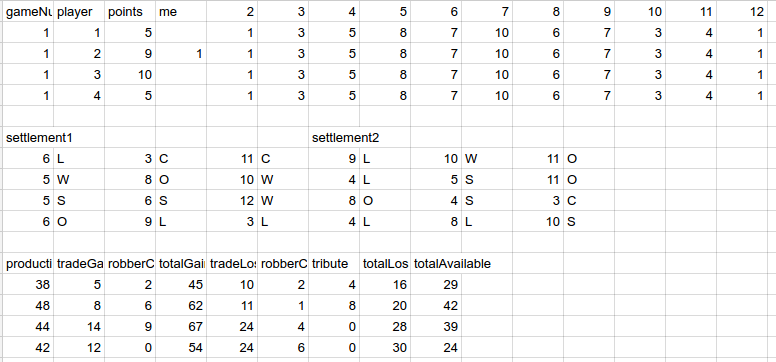
\includegraphics[width=0.8\textwidth]{data.png}
    \caption{Dataset snapshot}
    \label{fig:data}
\end{figure}

The dataset\footnote{https://www.kaggle.com/lumins/settlers-of-catan-games}
consists of data for 50 4-player games. Each game has 4 lines that consist
of starting position, points gained, placements of starting towns, total
resource gains and losses from production, robber cards and trade.

A snapshot of the dataset can be seen in figure \ref{fig:data}. We have mostly
used the data from the settlements and the points. The types of the attributes
can be seen in table \fig{tab:types}. It is worth nothing that the dices on
the resources are categorical because comparisons of them in this context is
meaningless. 

\begin{figure}
  \centering
  \begin{tabular}{|l|l|}
    Data & Type \\ \hline
    gameNum & Ratio \\ \hline
    player & Categorical \\ \hline
    points & Ratio \\ \hline
    me & Categorical \\ \hline
    #dice throws & Ratio \\ \hline
    Settlement:res & Categorical \\ \hline
    Settlement:dice & Categorical \\ \hline
    Gains & Ratio\\ \hline
    Losses & Ratio \\ \hline
  \end{tabular}
  \caption{Attribute types}
  \label{tab:types}
\end{figure}


To win a game of Settlers you need 10 points and there will never be two
players with 10 or more points at the same time. However it is possible to
finish the game with 11 or 12 points, but this skews the data without being
particularly interesting when determining a winner, so we changed all values
above 10 to just 10.

Generally points are the main indicator of success in the game, so whenever we
need to analyze the quality of combinations we will measure it against points.

\subsection{Visual encoding}

\section{Design}

\subsection{Illustration}
\includegraphics[scale=0.2]{pic.png}
\newpage
\noindent
The sketch shows on the left side a bunch of filters that you apply, once the user
have applied the filters on the right side will show a bunch of graphs of game statistics.
These graphs include how many points gained relative to which number or resource a player
had next to the starting settlements and other relevant statistics.
The filters that the user should be able to apply, includes which player position,
how many of a resource the start settlements started next to, gains and loses of resources,
numbers that start settlements lie up to and gains from the robber.

\subsection{Scenario of use}

A user wants to know whether it is a good idea to place settlements with no
access to clay. He skims through the list of visualization possibilities
and finds the resources tabs and chooses starts with "At most 0" of a
resource. A barchart is shown with 5 bars, one for each resource type. He
finds the clay bar and the task is complete.

\section{Implementation}
We plan on implementing the visualization using the d3 libary for data visualization.
For any needed pre-processing of the data we will use python.
\end{document}
